\documentclass[a4paper,10pt,twocolumn]{jsarticle}
\usepackage{docmute}
\usepackage{myjlababsstyle}
% \usepackage{fancyhdr}
% \usepackage{amsmath,amssymb}
% \usepackage{bm}
% \usepackage[dvipdfmx]{graphicx}
% \usepackage{subfigure}
% \usepackage{url}
% \usepackage{verbatim}
% \usepackage{wrapfig}
% \usepackage{ascmac}
% \usepackage{comment}
% \usepackage{lineno}
% %%%%%%%%%
% \usepackage{myjlababs}


\makeindex
\daigaku{青山学院大学}
\gakubu{社会情報学部}
%\gakka{社会情報学科}
\syubetsu{卒業研究}
%\labname{宮治研究室}
\chiefexaminer{宮治 裕 教授}

%%%%%%%%%%%%%%%%%%%%%%%%%%%%%%%%%%%%%%%
% ここから先「ここまで個人設定」の範囲に
% 各自の固有の情報を記入して下さい
%%%%%%%%%%%%%%%%%%%%%%%%%%%%%%%%%%%%%%%
\nendo{2021年度}
\snum{18118047} %学生番号
\jname{黒川 皇輝} %氏名
\thesistitle{感性空間を用いた画像の印象に合う楽曲推薦システムの開発} %タイトルを記入
\thesissubtitle{日本語の歌詞を用いた印象推定方法の評価} %サブタイトルを記入 ない場合はコメントアウト
\SUBTtrue %サブタイトル有りの場合 ない場合は,コメントアウト
%\SUBTfalse %サブタイトルなしの場合 有りの場合は,コメントアウト
%%%%%%%%ここまで個人設定%%%%%%%%%%%%%%%%%%

\begin{document}
%\linenumbers
\linesparpage{48} %行数指定
%\mojiparline{35} %文字数指定
\maketitle
\thispagestyle{pg}
\pagestyle{pg}

%%%%%%%%%%%%%%%%%%%%%%%%%%%%%%%%%%%%%%%
% ここから先「ここまで本文」の範囲に
% 各自の適切な抄録ファイルを読み込んでください
%%%%%%%%%%%%%%%%%%%%%%%%%%%%%%%%%%%%%%%
\documentclass[a4paper,10pt,twocolumn]{jsarticle}
\usepackage{myjlababsstyle}
\begin{document}
\section{はじめに}
近年Amazon Music,Spotifyといった音楽配信サービスとスマートフォンなどのモバイル端末の普及により,人々は膨大な楽曲を手軽に聴くことができるようになった.それに伴い音楽配信サービスのユーザは増加傾向にある\cite{1}.
膨大な楽曲の中からユーザが自身の嗜好に合う楽曲を見つけるのは困難であるため,楽曲を推薦するシステムが研究トピックとして着目されている.

ユーザの嗜好は時間と共に移り変わる.したがって,ユーザの気分や状況に合う楽曲を推薦するコンテキストアウェア楽曲推薦システムの需要が存在する.コンテキストは次のように定義されている.
「エンティティの状況を特徴化するのに用いられるあらゆる情報.エンティティとは,ユーザとアプリケーションとのインタラクションに関連する人や場所,オブジェクトを指し,それにはユーザ自身とアプリケーション自体も含まれる」\cite{2}.

テキストや映像,画像などの音楽以外のメディアからユーザが得る感性情報をマルチメディアコンテキストという.
マルチメディアコンテキストの観点から,歌詞からユーザが受ける印象を推定する研究が行われている.しかし,いまだ確立された手法は存在していない.

本研究では日本語歌詞から読み取れる印象を推定する手法の設計と評価をする.
%
\end{document}
\documentclass[a4paper,10pt,twocolumn]{jsarticle}
\usepackage{myjlababsstyle}
\begin{document}
\section{関連研究}
角田ら(2018)\cite{4}は印象をPlutchikの感情モデルの基本8感情\cite{5}を用いて推定した.形態素解析ツールを用いて歌詞から単語を抽出する.その後Word2Vecを利用してのベクトル変換を行ない,
基本8感情との類似度を算出して,一番類似度が高い感情をテキストから得られる印象とした.この研究では喜び,悲しみなどの推定できた印象と嫌悪,怒りなどの推定できなかった印象が存在した.

大木ら(2018)\cite{6}は日本語評価極性辞書にのっとり,歌詞をポジティブ・ネガティブ・ニュートラルの3つの印象に分類した.3つの評価極性を歌詞内の各単語に付与し,単語の評価極性値を平均化することで歌詞自体への印象の評価値を算出する.
歌詞をポジティブ,ネガティブ,ニュートラルの3印象にうまく推定できるが,より詳細な印象(喜び,悲しみなど)は正確に推定できていない.

上記で述べたとおり,歌詞情報から印象を推定する研究は未だ発展途上であるため,Word2Vecや日本語評価極性辞書以外で印象推定する手法を模索する.
西川らは英語の感情価単語セットANEW\cite{7}を用いて,歌詞をAV平面上で表現する研究を行なった.歌詞の各フレーズが持つ単語のAV平面座標を推定して,フレーズごとの平面座標を求めた.
この印象推定手法は英語の歌詞を用いて効果測定が行われたが,日本語の歌詞での効果測定は行われていないので,日本語の歌詞の場合でもこの手法が効果を発揮するのか調査する.
本間ら\cite{8}はANEWの単語を参考にして,日本語訳した単語セットを作成した.
よって,この日本語の単語セットを利用すれば,西川らが考案した手法を日本語の歌詞の印象推定でも一定の効果を挙げられることが予想される.

%
\end{document}

\documentclass[a4paper,10pt,twocolumn]{jsarticle}
\usepackage{myjlababsstyle}
\begin{document}
\section{歌詞印象推定手法}
\subsection{印象の定義}
本稿で推定する印象とはRussellのAV平面上で表現する.AV平面は縦軸にArousalを,横軸にValenceを取る2次元平面である.Arousal軸は正の方向に興奮を,負の方向に弛緩を表す.そして,Valence軸は正の方向に快を,負の方向に不快を表す.
AV平面の4象限は第1象限から順に喜怒哀楽の印象を表す.

\subsection{歌詞データの収集}
歌詞データの収集はUta-Net\footnote{https://www.uta-net.com/}から人気のアーティストの曲を6,813曲収集した.本研究では6,813曲から3,000曲を無作為に選んだ.

\subsection{ANEWデータの拡張}
本間らが開発した日本語版ANEWの単語の類義語と同義語をWordNet\cite{10}を用いて探索する.発見した単語に類義語元の単語が持つArousalとValenceの値を与えることで,日本語版ANEWを14,232語に拡張した単語データセットを日本語版ANEW拡張データセットとする.
日本語版ANEW拡張データセットの構成はA+V+平面に5,581語,A+V--平面に2,681語,A--V--平面に3,456語,A--V+平面に2,493語である.

\subsection{歌詞データの整形}
収集した歌詞データの中に一部英語が入っていたので,英語の歌詞を削除した.そして歌詞データを歌詞のフレーズごとに分解した.形態素解析器MeCabを用いて各フレーズから名詞・形容詞・動詞を抜き出した.歌詞から抜き出した単語の総数は109,450語である.

\subsection{歌詞印象推定}
確率的潜在意味解析(PLSA)を利用する.歌詞のフレーズを文書dとし,フレーズ中に出現する単語を単語wと定義してモデルパラメータを推定した.
P(w\verb+|+z)はトピックから単語が観測される確率であるため,この確率の高い単語がトピックを表現する.
歌詞の印象を推定するためには潜在的なトピックzを印象に制限する必要がある.通常のPLSAは文書と単語の共起確率に着目して,潜在的なトピックを推定する手法であるため,必ず潜在的なトピックが印象を表現するとは限らない.
よって,日本語版ANEW拡張データセットを事前知識として使用し,モデルパラメータをMAP推定することで潜在的なトピックにAV平面の各象限を表現する.
具体的に潜在的なトピックzを次の式(1)のようにAV平面の各印象として定義する.
\begin{equation}
\rm{z\in\{A+V+,A+V-,A-V-,A-V+\}}
\end{equation}
モデルパラメータP(w\verb+|+z)の対数事前分布を共役事前分布を用いて式(2)に定義する.kは出現する単語の集合を表す.
\begin{equation}
\rm{log P(θ)\propto\sum_k\sum_z(\alpha_{w_k,z}-1)\log P(w_k|z)}
\end{equation}
共役事前分布のハイパーパラメータαは日本語版ANEW拡張データセットに含まれる単語で該当の象限に位置する場合のみ原点からの距離を入力する.それ以外の場合無情報事前分布を与える.
ラグランジュの未定乗数法を使用して対数尤度関数と対数事前分布よりMAP推定値を求める
MAP推定値は式(3)で表す.
\begin{equation}
\rm{P(w_k|z)_{map}=\frac{\alpha_{w_k,z}-1+p(w_k|z)}{1-K+\sum_k\sum_z\alpha_{w_k,z}}}
\end{equation}
P(z)とP(d\verb+|+z)の推定には無情報事前分布を与えた.
ベイズの定理よりP(z\verb+|+w)は式(4)で求められる.
\begin{equation}
\rm{P(z|w_k)=\frac{P(w_k|z)_{map}P(z)}{P(w_k)}}
\end{equation}
各フレーズdのArousalとValenceの値は求めたP(z\verb+|+w)を用いて求めた各単語wのArousalとValenceの値を合計.正規化して求める.
以上で歌詞中のフレーズごとに感情価を求める.

%
\end{document}
\documentclass[a4paper,10pt,twocolumn]{jsarticle}
\usepackage{myjlababsstyle}
\begin{document}
\section{実験}

%
\end{document}

\documentclass[a4paper,10pt,twocolumn]{jsarticle}
\usepackage{myjlababsstyle}
\begin{document}
\section{その他}
その他の事項として、本節では表の記述方法とぶち抜きの図について記載する。

\subsection{表の記述}
論文を記述する際にも指摘したが、表においては数値は右詰にしなければならない。
また、ラベル部は中央揃えとすることが多い。

そのような設定をしたものを、表~\ref{table:face_rec}に示す。

\begin{table}[b]
\centering
\vspace{2mm}
\caption{WHLACによる顔表情認識率}
\label{table:face_rec}
\vspace{3mm}
\small
\begin{tabular}{r|r|r|r} \hline
\multicolumn{1}{c|}{Data \#} & \multicolumn{1}{c|}{Ave.} & \multicolumn{1}{c|}{Max.} & \multicolumn{1}{c}{Min.} \\ \hline\hline
1 &  0.67 (N/A) & 0.91 (39) & 0.46(21) \\ \hline
2 & 0.37 (N/A) & 0.50 (38) & 0.09(10) \\ \hline
3 & 0.65 (N/A) & 0.87 (45) & 0.28(10) \\ \hline\hline
\multicolumn{1}{c|}{Total Ave.} & 0.56 & 0.76 & 0.27 \\ \hline
\end{tabular}
\end{table} %

\subsection{二段ぶち抜きの図}
二段組の省略ではあるが、図表の設定(開始タグと終了タグを共に)を~\verb+figure*+ とすることで、左右の段をぶち抜いて図表を入れることができる。
例を図\ref{fig:mp2}に示す。

\begin{screen}
{\small
\begin{verbatim}
\begin{figure*}[bt]
\centering
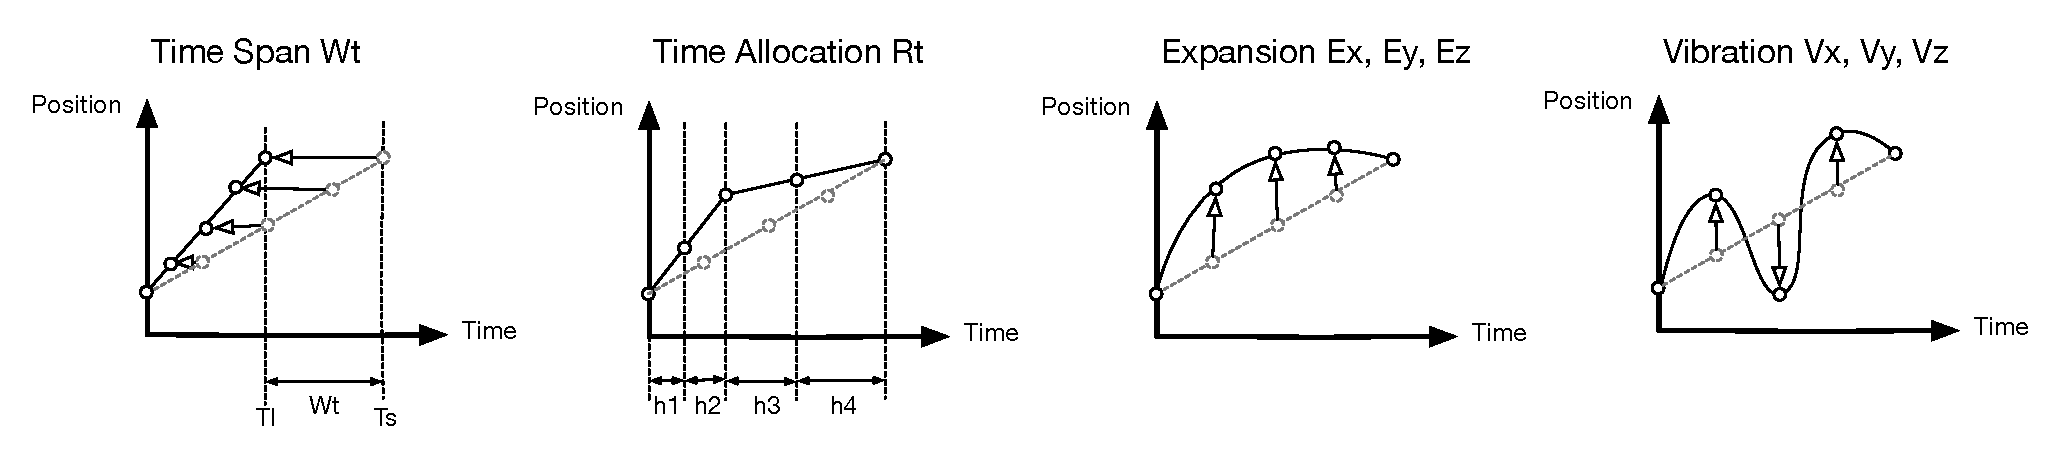
\includegraphics[width=14cm]{mp2.pdf}
\vspace{-7mm}
\caption{MMSの内部構成}
\label{fig:mp2}
\vspace{5mm}
\end{figure*}
\end{verbatim}
}
\end{screen}

\begin{figure*}[bt]
    \centering
    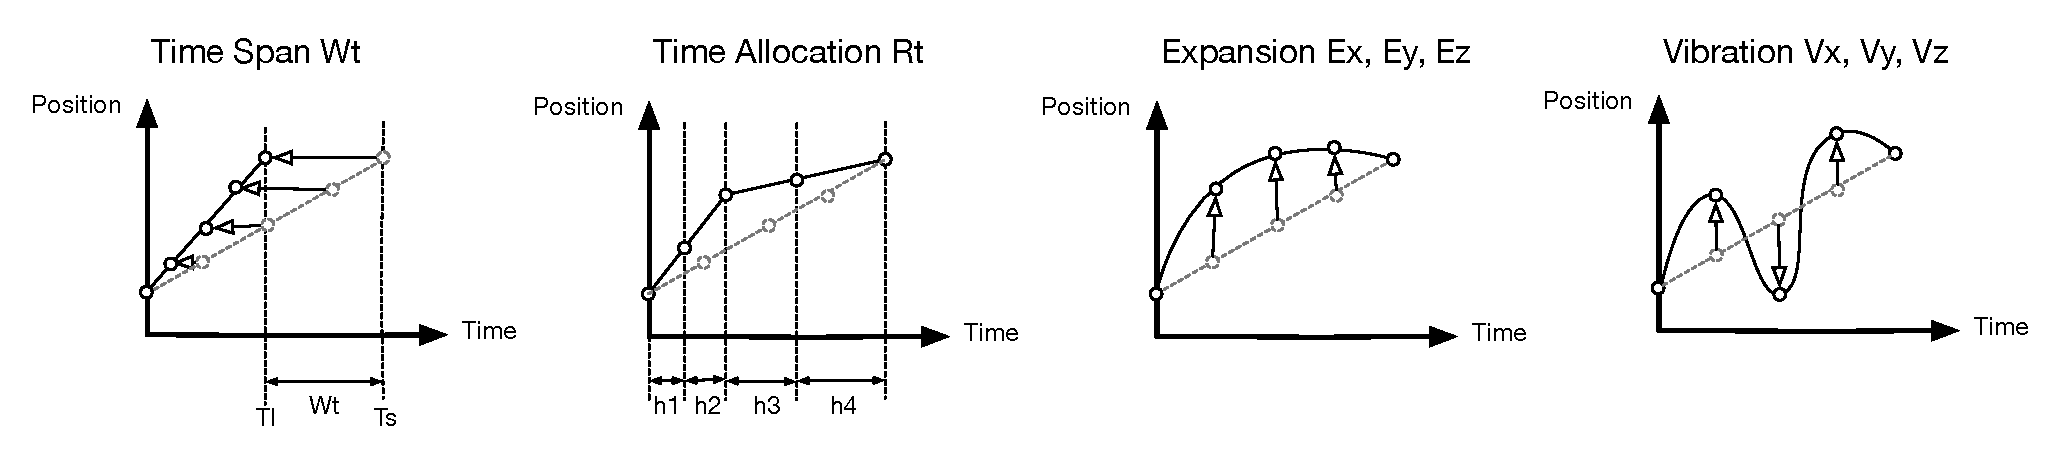
\includegraphics[width=18cm]{mp2.pdf}
    \vspace{-7mm}
    \caption{MMSの内部構成}
    \label{fig:mp2}
    \vspace{5mm}
\end{figure*}



%
\end{document}
\documentclass[a4paper,10pt,twocolumn]{jsarticle}
\usepackage{myjlababsstyle}
\begin{document}
\section{Visual Studio Codeで編集する人へ}
Visual Studio Codeを使って \LaTeX 論文を作成する人が増えているため、それに合わせた修正を各所でおこなっている。
以下の設定や、注意事項を参照してほしい。

\subsection{コンパイルのための設定}
\LaTeX をコンパイルする際には、目次や参照、参考文献などを組み込むための処理などを複数回実行する必要がある。
これを自動で判断して実行するための設定ファイルが \verb+.latexmkrc+である。
本スタイルファイルパッケージでは、以下の設定をしている。
\begin{screen}
{\small
\begin{verbatim}
#!/usr/bin/env perl
$pdf_mode = 3;
$latex = 'platex -halt-on-error';
$bibtex = 'pbibtex';
$dvipdf = 'dvipdfmx %O -o %D %S';
\end{verbatim}    
}
\end{screen}

なお、一部の行を割愛して表示している。
詳細は、直接ファイルを確認してほしい。

\subsection{LaTeX Workshop の設定}
VSCodeプラグインであるLaTeX Workshopの設定は、以下の様にしている。
なお、必ずしも同じ設定にする必要はない。
\begin{screen}
{\footnotesize
\begin{verbatim}
"latex-workshop.latex.tools": [
  {
    "name": "Latexmk (pLaTeX)",
    "command": "latexmk",
    "args": [
      "-f",
      "-gg",
      "-pv",
      "-latex='platex'",
      "-synctex=1",
      "-interaction=nonstopmode",
      "-file-line-error",
      "%DOC%"
    ]
  },
],
\end{verbatim}
}
\end{screen}
\begin{screen}
    {\footnotesize
    \begin{verbatim}
"latex-workshop.latex.recipes": [
  {
    "name": "pLaTeX",
    "tools": [
      "Latexmk (pLaTeX)"
    ]
  },
],
\end{verbatim}
}
\end{screen}
\begin{screen}
{\footnotesize
\begin{verbatim}
"latex-workshop.latex.magic.args": [
  "-f",
  "-gg",
  "-pv",
  "-synctex=1",
  "-interaction=nonstopmode",
  "-file-line-error",
  "%DOC%"
],
\end{verbatim}
}
\end{screen}
\begin{screen}
{\footnotesize
\begin{verbatim}
"latex-workshop.view.pdf.viewer":"tab",
"latex-workshop.latex.autoBuild.run": "never",
"latex-workshop.view.pdf.refviewer":"tabOrBrowser",
"latex-workshop.latex.autoClean.run":"onBuilt",
\end{verbatim}
}
\end{screen}

\subsection{分割(子ファイル)コンパイル}
通常の \LaTeX のファイルの場合に親ファイルに記述する文書開始や終了/スタイルファイルの読み込みを子ファイル側に書き込むことによって、それぞれのファイルごとにコンパイルができる。

\begin{screen}
{\footnotesize
\begin{verbatim}
\documentclass[a4paper,10pt,twocolumn]{jsarticle}
\usepackage{myjlababsstyle}
\begin{document}
\section{これは読み込まれる子ファイルの例}
ファイル名は sub.tex とします。
\end{document}
\end{verbatim}
}
\end{screen}

これを読み込む親ファイル側では、これらの設定を無視するようにしなければならない。
そのために、\verb+docmute+パッケージを用いている。
親ファイルの例を以下に示す。
\begin{screen}
{\footnotesize
\begin{verbatim}
\documentclass[a4paper,10pt,twocolumn]{jsarticle}
\usepackage{docmute}
\usepackage{myjlababsstyle}
\begin{document}
これは親ファイルの例です。
\input{sub}
\end{document}
\end{verbatim}
}
\end{screen}

また、多くのスタイルファイルを親ファイルと子ファイルで共通して読み込むために、スタイルファイルを \verb+myjlababsstyle.sty+ ファイル内に列挙している。
各自でスタイルファイルを追加する場合には、このファイルに記載すること。

\subsection{テキスト校正くん}
「テキスト校正くん」パッケージは追加すべきである。
ただし、\LaTeX のファイルは校正してくれないため、\verb+txt+か\verb+md+のファイルを作成し、そこに文章を貼り付けて校正するのが良い。
インストールや設定などが必要ない「テキスト校正くん」を利用することにしたが、昨年まではRedpenと比較して細かい部分の校正は不十分である。
最低限の校正として必ず利用してほしい。
%
\end{document}
\documentclass[a4paper,10pt,twocolumn]{jsarticle}
\usepackage{myjlababsstyle}
\begin{document}
\section{システム構成図の例}
システム構成図が論理的に描けると、論文そのものの説明もしやすくなる。
ここでは、シスム構成図の例をいくつか記載する。
\begin{figure}[t]
  \centering
  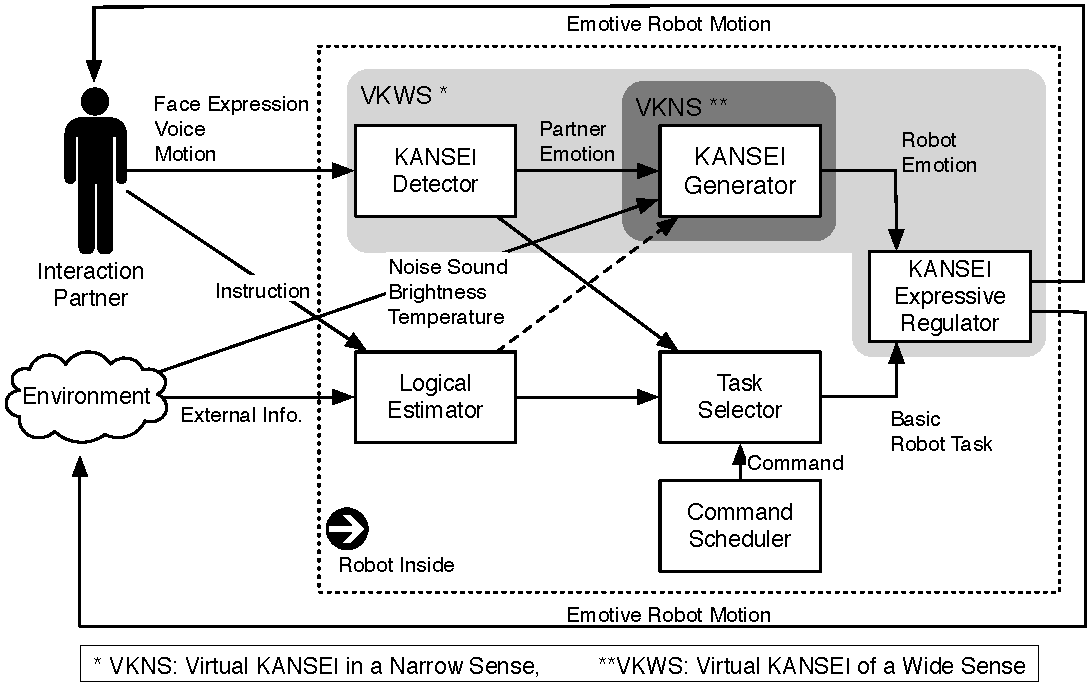
\includegraphics[width=9cm]{VKall.pdf}
  \vspace{-7mm}
  \caption{擬似感性の構成}
  \label{fig:vkall}
  \vspace{5mm}
\end{figure}

\begin{figure}[t]
  \centering
  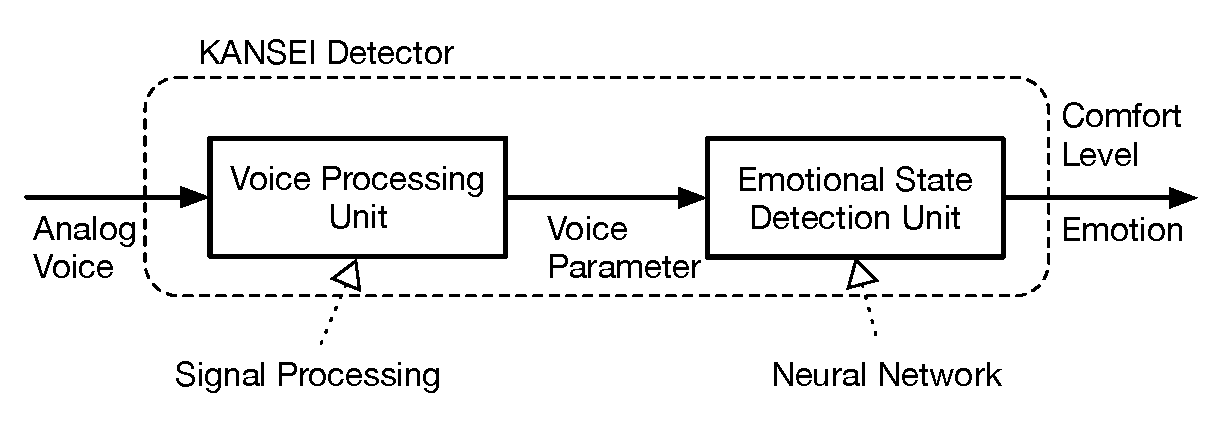
\includegraphics[width=8cm]{VoiceKANSEIDetector.pdf}
  \vspace{-7mm}
  \caption{音声からの感性同定部}
  \label{fig:VoiceKANSEIDetector}
  \vspace{5mm}
\end{figure}

%
\end{document}

%%%%%%%%ここまで本文%%%%%%%%%%%%%%%%%%%%%%

\bibliographystyle{junsrt}
\bibliography{myrefs}
% myrefs.bib の中はサンプルファイルを参考に記述
%
\end{document}
